\documentclass[12pt,border=4pt]{standalone}
\usepackage{tikz}
\usetikzlibrary{arrows.meta,positioning,shapes.geometric,fit,backgrounds,calc}
\begin{document}
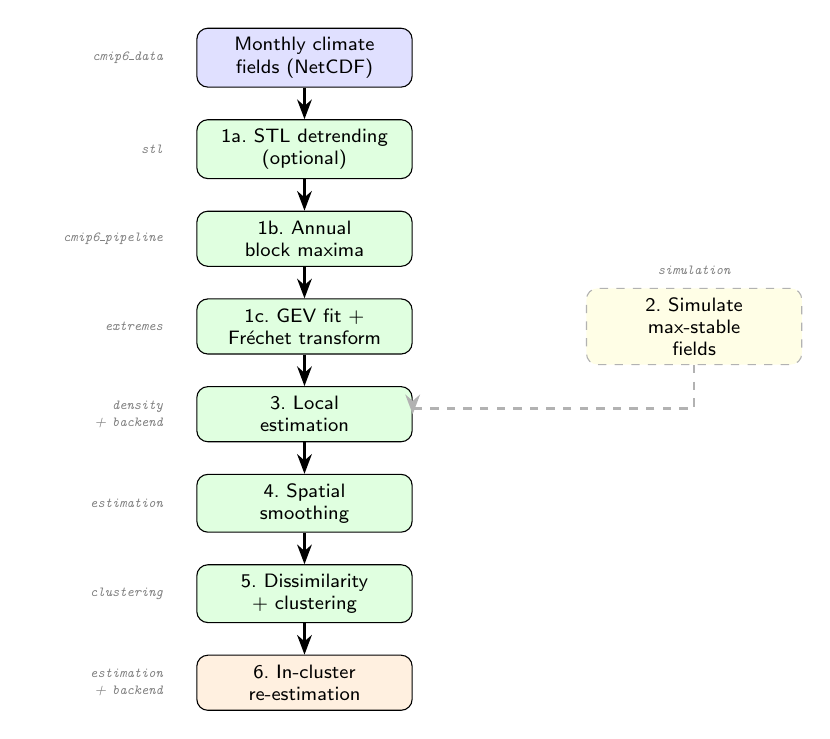
\begin{tikzpicture}[
  box/.style={draw, rounded corners=4pt, minimum width=2.6cm,
    minimum height=0.7cm, font=\sffamily\scriptsize,
    align=center, text width=2.5cm},
  data/.style={box, fill=blue!12},
  proc/.style={box, fill=green!12},
  outbox/.style={box, fill=orange!12},
  simbox/.style={box, fill=yellow!10, draw=gray!60, dashed},
  arr/.style={-{Stealth[length=2.5mm]}, thick},
  arrdashed/.style={-{Stealth[length=2.5mm]}, thick, dashed, gray!60},
  note/.style={font=\itshape\tiny, text=gray},
  node distance=0.4cm,
]

\node[data] (raw) {Monthly climate\\fields (NetCDF)};

\node[proc, below=of raw] (stl)
  {1a.\ STL detrending\\(optional)};
\node[proc, below=of stl] (bm)
  {1b.\ Annual\\block maxima};
\node[proc, below=of bm] (frech)
  {1c.\ GEV fit +\\Fr\'{e}chet transform};
\node[proc, below=of frech] (mle)
  {3.\ Local\\estimation};
\node[proc, below=of mle] (smooth)
  {4.\ Spatial\\smoothing};
\node[proc, below=of smooth] (clust)
  {5.\ Dissimilarity\\+ clustering};
\node[outbox, below=of clust] (out)
  {6.\ In-cluster\\re-estimation};

\draw[arr] (raw) -- (stl);
\draw[arr] (stl) -- (bm);
\draw[arr] (bm) -- (frech);
\draw[arr] (frech) -- (mle);
\draw[arr] (mle) -- (smooth);
\draw[arr] (smooth) -- (clust);
\draw[arr] (clust) -- (out);

\node[simbox, right=2.2cm of frech] (sim)
  {2.\ Simulate\\max-stable\\fields};
\node[note, above=0.05cm of sim, text width=2.5cm, align=center]
  {\texttt{simulation}};
\draw[arrdashed] (sim.south) -- ++(0,-0.55) -| (mle.east);

\node[note, left=0.3cm of raw, text width=1.6cm, align=right]
  {\texttt{cmip6\_data}};
\node[note, left=0.3cm of stl, text width=1.6cm, align=right]
  {\texttt{stl}};
\node[note, left=0.3cm of bm, text width=1.6cm, align=right]
  {\texttt{cmip6\_pipeline}};
\node[note, left=0.3cm of frech, text width=1.6cm, align=right]
  {\texttt{extremes}};
\node[note, left=0.3cm of mle, text width=1.6cm, align=right]
  {\texttt{density}\\+ \texttt{backend}};
\node[note, left=0.3cm of smooth, text width=1.6cm, align=right]
  {\texttt{estimation}};
\node[note, left=0.3cm of clust, text width=1.6cm, align=right]
  {\texttt{clustering}};
\node[note, left=0.3cm of out, text width=1.6cm, align=right]
  {\texttt{estimation}\\+ \texttt{backend}};

\end{tikzpicture}
\end{document}
